\chapter{相关工作}
\label{cha:relatedwork}
本章将主要对渲染算法的重要技术进行简单的介绍。
由于研究的内容同时涉及光线追踪的并行化技术与部分机器学习相关算法,
因此也会对这些领域的工作进行部分整理。

\section{渲染算法}

正如上一章所提到的,渲染技术从提出至今已经拥有超过50余年的历史,已经是一门相当成熟的学科。

%^ Immel, David S.; Cohen, Michael F.; Greenberg, Donald P. (1986), "A radiosity method for non-diffuse environments" (PDF), Siggraph 1986: 133, doi:10.1145/15922.15901, ISBN 978-0-89791-196-2
%^ Kajiya, James T. (1986), "The rendering equation" (PDF), Siggraph 1986: 143–150, doi:10.1145/15922.15902, ISBN 978-0-89791-196-2
%Watt, Alan; Watt, Mark (1992). "12.2.1 The path tracing solution to the rendering equation". Advanced Animation and Rendering Techniques: Theory and Practice. Addison-Wesley Professional. p. 293. ISBN 978-0-201-54412-1.
%Kajiya, James T.; Von Herzen, Brian P. (1984), "Ray tracing volume densities", Siggraph 1984, 18 (3): 165, CiteSeerX 10.1.1.128.3394, doi:10.1145/964965.808594

渲染技术有着完整而牢固的理论基础。
由David Immel等人\cite{RenderingEquation1},以及James Kajiya\cite{RenderingEquation2}在1986年同时提出的渲染方程,被认为是最著名的渲染理论之一:
\begin{equation}
    L_o(\mathbf{x}, \omega_o)=L_e(\mathbf{x},\omega_o)+\int_{\Omega} f(\mathbf{x}, \omega_i, \omega_o) L_i(\mathbf{x}, \omega_i) (\omega_i \cdot \mathbf{n}) \operatorname d\omega_i
\end{equation}
该方程利用物理方法近似描述了在几何光学模型(即不考虑光的波长效应)中光照辐射度的传输形式,成为了后来大量渲染算法的理论来源。
1992年Alan Watt等人进一步得出,渲染方程是Fredholm积分中的第二类积分\cite{Fredholm}。
除此之外,针对不同种类的渲染需求,许多相对应的理论也先后被提出,
如James Kajiya等人在1984年曾提出体渲染方程\cite{VolumnRenderingEquation},主要运用于传输介质非真空情况下的体渲染;
Adam M Smith等人提出的短时渲染方程\cite{TransientEquation},用于渲染Time-Of-Flight类型图像等等。



在确定渲染的目标是求解渲染方程后,许多至今仍在沿用的渲染算法相继出现。
按照工作原理,这些算法大致可以分为基于光线追踪的渲染算法和基于光栅化的渲染算法。   
事实上,它们的算法框架早在渲染方程提出之前就都已经形成,
然而时至今日,这些算法绝大多数都以该方程作为其理论基础。
下面将对它们进行更加详细的介绍。

\subsection{基于光线追踪的渲染算法}

所谓光线追踪,便是通过相机通过各个角度向外发射光线,并通过递归算法对光线进行跟踪
,从而获得包含反射、折射效果的渲染图像的方法。
通常认为,最早提出的光线追踪算法是由Arther Appel在1968年提出的光线投射算法\cite{RayCasting}。
然而,该算法仅完成了光线追踪流程中的第一步,相机发射的光线在与物体相交之后便直接求得光照值。
真正意义上完整的光线追踪算法,则最早由Turner Whitted于1979年提出,名为递归式光线追踪算法\cite{WhittedRayTracing}(也被称作Whitted风格的光线追踪算法)。
该算法也首次提出了次级光线这一名词,用来表示当前光线与物体表面交互而形成的新光线。

\begin{figure}[h]
    \centering
    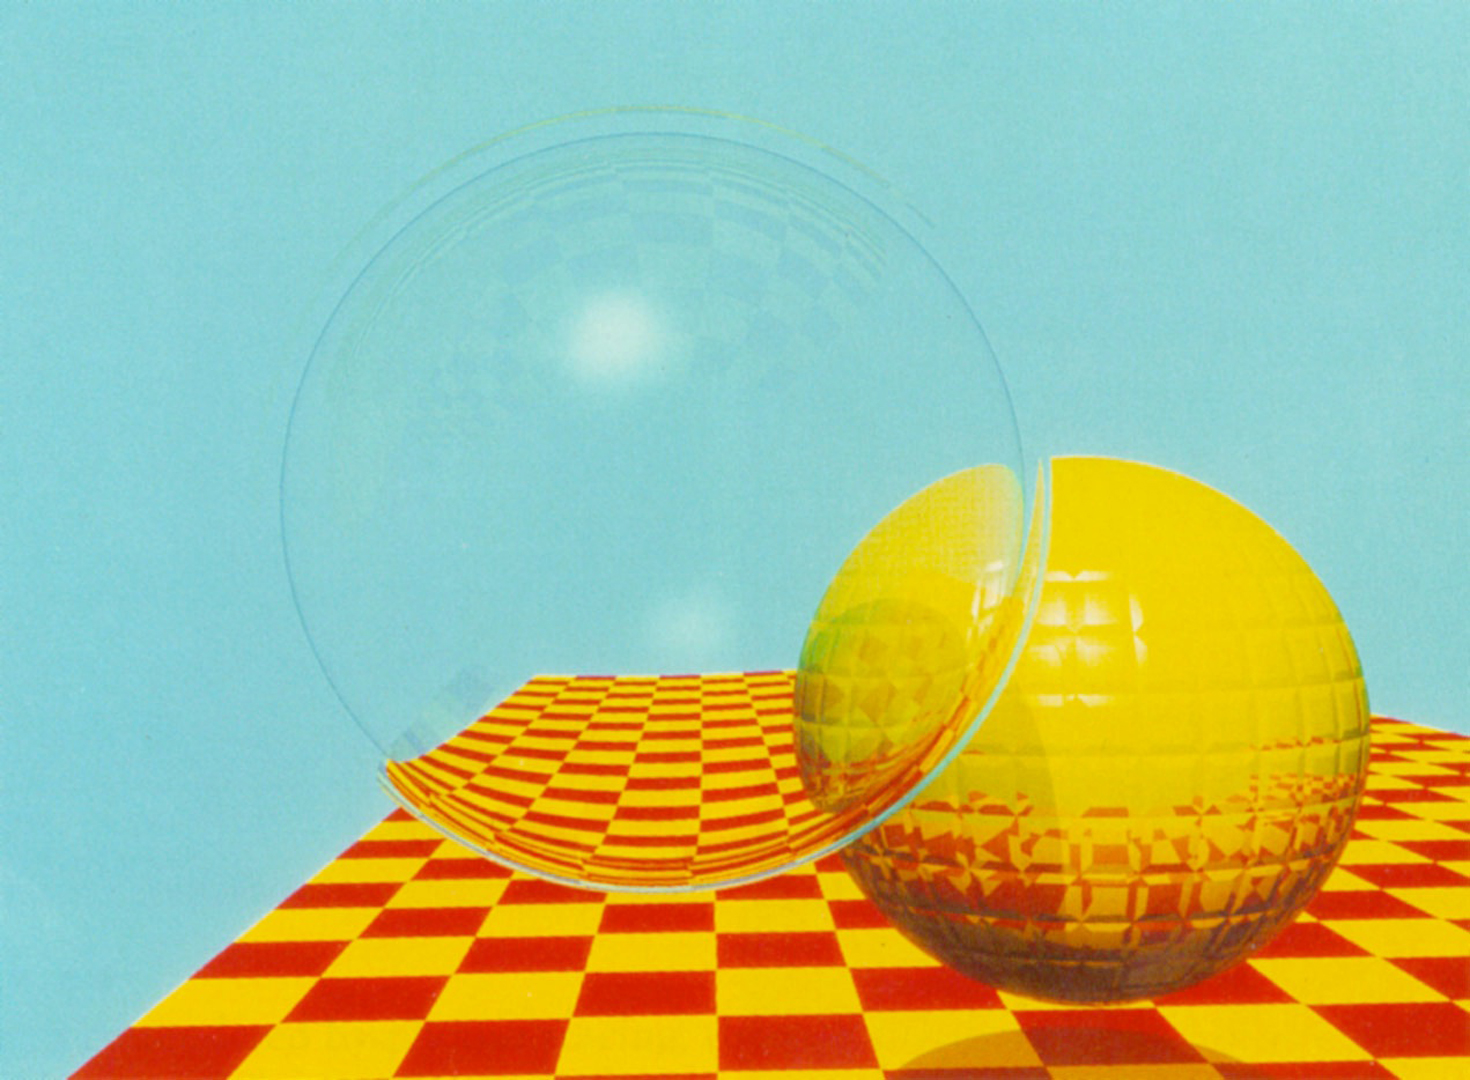
\includegraphics[height=3.5in]{RayTracing.jpg}
    \caption{利用递归式光线追踪算法生成的图像}
    \label{tab:rayTrace}
\end{figure}

递归式光线跟踪算法能够支持结构复杂的场景,但是仍然存在一点明显的不足:
算法生成的光线与次级光线都有着确定的路径,这样可能会带来严重的锯齿问题,
且无法实现软阴影、运动模糊等类似的“软”效果。
为了改进这点缺陷,1984年由Robert Cook提出的分布式光线追踪算法\cite{DistributiveRayTracing}首次在光线生成上加入了不确定性,
并引入了随机采样的机制。
%http://artis.inrialpes.fr/Enseignement/TRSA/CookDistributed84.pdf
% figure 

1986年,在渲染方程问世后不久,其提出者James Kajiya很快又提出了路径追踪算法\cite{PathTracing},
这一算法与相比之前增加了几点重要的创新:
首先引入了蒙特卡洛积分法来求解渲染方程,并提出了基于物体BRDF的采样函数;
其次将以往路径追踪算法中存储光线的树结构变为了多条单一的路径结构。
由于理论性质的完善,路径追踪算法被认为是第一个“无偏”的光线追踪算法,
其实际的运行效果也比以往有了巨大的提升。
% figure

\label{PathTracingOptimization}
路径追踪算法尽管获得足够精确的计算结果,却在收敛速度上较为缓慢。
为了提升收敛速度,有许多针对路径追踪的优化算法被提出。其中,
一部分算法试图从采样方式上进行优化,如Veach and J.Guibas于1995提出的复合重要性采样\cite{MultipleImportanceSampling}算法,
通过从多个不同的分布进行联合采样的策略,来减小一些场景的误差;
William J. Morokoff等人在1995年提出拟蒙特卡洛积分法\cite{QuasiMonteCarlo},
利用固定的序列代替伪随机数从而减小估计值的方差,这一思路同样被运用到了路径追踪算法中;
许多工作\cite{Belcour2013}\cite{AdaptiveSampling}试图通过已有的渲染结果来选择接下来的采样密度分布,这些算法又被统称为适应性采样。
有的算法则直接对路径追踪生成的图片进行过滤,从而起到降噪效果,这其中的工作包含有:
TODO:[Sen and Darabi, 2011], [Kalantari et al. 2015], [Rousselle et al. 2011]等等。

相较于优化算法中的某些具体步骤,另一些工作则考虑如何对算法本身做出改进。
Lafortune在1996年提出的双向路径追踪算法\cite{BidirectionalPathTracing}便是典型的代表之一,
其基本思路是在每轮迭代中,同时从摄像机与光源各发射并追踪一条光线,然后在两条路径上的节点两两之间分别计算光照。
这一算法有效地降低了渲染误差,且使得许多在原算法中难以追踪到的路径也能被计算。

对于如何处理从光源发射的光线,和双向路径追踪算法不同的另一条思路是,
将这些光线信息直接存储在场景的物体表面上,然后通过统计一定范围内的光线的数量,
来获取表面上任意一点实际光照亮度的近似值。这类思路所主导的算法被称为光子映射算法,而上述的光线也被称为光子。
光子映射算法最早出现在1993年(TODO:谁的工作?),而在此之后又受到多次改良。
Toshiya Hachisuka等人于2008年提出了渐进式光子映射算法\cite{ProgressivePhotonMapping},
大大缩小了算法所需要的内存空间和运行时间复杂度;
仅一年之后,Toshiya Hachisuka等人又发表了随机渐进式光子映射算法\cite{StochasticProgressivePhotonMapping},
利用光子也得以计算出之前所提到的各类“软”效果。

除了上述提到的所有算法之外,著名的光线追踪渲染算法还包括
MLT算法、顶点连接与合并算法等等,这里就不一一进行介绍了。


\subsection{基于光栅化的渲染算法}

按照严格定义,所谓光栅化其实是指是图形渲染管线中,将输入场景中的几何数据(又名顶点数据)转换为片元数据(从而对应到屏幕中的各个像素点)的过程。
对于大多数采用管线的渲染算法而言,光栅化都是不可或缺的一个关键步骤,因此这一类渲染算法也被称之为光栅化渲染。

TODO:算法理论
%Siggraph 1985 - "Fast Spheres, Shadows, Textures, Transparencies, and Image Enhancements in Pixel-Planes," Henry Fuchs,et. al.
%2000 Sig/Euro Workshop on Graphics Hardware - "Tiled Polygon Traversal Using Half-Plane Edge Functions," Joel McCormack, Robert McNamara
%Siggraph 1988 - "A Parallel Algorithm for Polygon Rasterization,"  Juan Pineda
%Siggraph 2005 - “Resolution-Independent Curve Rendering Using Programmable Graphics Hardware,” Charles Loop, Jim Blinn

和光线追踪算法不同的一点是,光栅化渲染算法不仅仅针对三维场景的渲染,
而同样可以用于二维场景、图形界面等其他需求,具有更加广泛的适应性。
除此之外,光栅化渲染由于拥有通过固定的流水线完成并行计算,
因此速度相比前者快上许多,几乎被当前所有的实时渲染技术所采用。
然而,光栅化算法也有自身的弱势。光栅化算法并没有在渲染中对次级光线进行跟踪,
加之对于实时渲染而言,运行时间上有着严格限制,因此在效果上的表现一般会差于光线追踪算法。
为了弥补这一点缺失,有大量的技术试图采用近似的方法来达到更加真实的效果。
这些技术普遍采用的思路是将复杂的光学方程进行拆分,
把所求光照值分解成多个容易计算,或可以通过预处理得到的组成部分,再通过叠加形成最终的图像。

这些技术中,有的着力于计算渲染中产生的阴影效果\cite{AO},有的将中心放在全局光照计算上\cite{GI},
有的则研究如何快速对体渲染中的效果进行近似\cite{Volume}。
事实上,由于来自工业界(尤其是娱乐行业为首)的需求之庞大,
基于光栅化的渲染技术(或者实时渲染技术)在很长时间来都属于相当热门的研究课题。
正因如此,该技术的发展速度相当迅速,与之相关的工作浩如烟海,从而也出现了不少专门对相关算法进行整理介绍的书籍。
其中,较为有名的包括《Real-time Rendering》\cite{RealTimeRendering},《Physically-Based Rendering》\cite{PhysicallyBasedRendering}(又名PBR)
等书,都已经成为该领域中的经典之作,对目前的渲染行业产生了深刻的影响。


\section{光线追踪渲染的并行化}

自从光线追踪框架被提出以来,便有很多学者对其并行化产生了强烈兴趣。
按照硬件基础的不同,并行化光线追踪技术可以分为两种:
第一种是基于CPU的并行技术,主要通过多CPU机器、多核CPU、网络以及分布式系统实现并行;
第二种是基于GPU的并行技术,通过GPGPU的通用并行计算功能来实现光线追踪框架。
下面将对两种技术依次进行介绍。

\subsection{基于CPU的并行化}

如果不考虑运行机器规模的限制的话,早期的许多相关工作便已经在速度上达到了惊人的水平。
1982年,由Osaka University带领的团队利用
一台含有514个处理器的大型并行计算机LINKS-1达到了极快的渲染速度\cite{LINKS1},
因此也是最早被称做实时的光线追踪渲染器。
LINKS-1计算机拥有空前的巨大规模,直到1984年仍然是世界上能力最强的计算机之一。

尽管这项工作在效果上表现出色,但由于其所用的机器过于庞大,因此很难继续拓展下去。
1986年,Mike Muuss在设计BRL-CAD时另辟蹊径,试图采用网络链接的分布式系统实现并行化,
同样取得了良好的运行效果(速度达到了每秒一帧以上)\cite{BRLCAD}。

更进一步地,人们开始期望实时光线追踪在体型普通的单台机器上运行。于是一方面,
渲染界的学者们开始思考如何尽可能减少算法的运算量,而另一方面,
CPU的设计者们也在不断设计更强大的芯片架构,使其逐渐满足光线追踪算法的运算需求。
直至2008年,Intel公司在一次展示中,
利用一款包含16核处理器的Xeon Tigerton系统完成了720p分辨率下的实时光线追踪,
刷新频率则达到了14-29赫兹\cite{QuakeWars}。

然而在此之后,随着CPU速度的提升逐渐放缓,基于CPU的并行光线追踪技术也最终遇到
了发展瓶颈。于是,学者们开始将目光转移到原本用于光栅化渲染的图形处理器上,
探求通过另一种硬件来实现这一目标。

\subsection{基于GPU的并行化} 

早在2002年,Tim Purcell便首次提出了通过GPU实现的全局光照算法,为后来GPU光线追踪的出现埋下了萌芽。
2009年,来自Nvidia公司的Austin Robison展示了首个在GPU上运行的路径追踪渲染器,
很快过后,Nvidia公司便正式向外公布了对后来影响巨大的GPU光线追踪库——OpTiX\cite{Optix}。

TODO:OpTiX的一张示意图

OpTiX的问世归功于不断走向成熟的通用图形处理器(GPGPU)。
相比原本的GPU而言,GPGPU拥有者两点至关重要的特性:
首先,它不存在管线编程的限制,这使得光线追踪里例如采样,计算反射光等复杂操作都能被实现;
其次,也是最为关键的一点,便是在较为成熟的GPGPU中,内核程序也拥有调用函数的能力,因此可以实现递归操作。这是光线追踪算法的核心需求所在。

在此之后的时间内,利用GPU实现实时光线追踪的热度一路上涨,一些商用化的成果也慢慢呈现出来。
AMD公司利用自己研发的GPUOpen Radeon ProRender渲染器,在自家的Vega系列GPU上启用了实时光线追踪功能\cite{Vega};
NVIDIA公司在新发布的GeForce 20系列显卡中,加入了名为RTX的实时光线追踪功能\cite{RTXOn}。
越来越多的游戏诸如《战地5》,《我的世界》等,也已经开始实际应用起该项技术。

\section{机器学习与渲染}

机器学习和渲染技术有着密不可分的联系。为渲染而诞生的图形处理器
加速了机器学习的发展,而逐渐趋向成熟的后者又反过来对渲染产生了积极影响。
在计算机视觉领域,考虑到精确标注的现实数据往往不易取得,
近年来许多工作尝试用利用渲染技术生成合成数据,同样取得了良好的效果。
下面将对一些渲染中的机器学习算法和基于渲染的数据生成相关工作进行介绍,

\subsection{用于渲染的机器学习算法}

正如\ref{PathTracingOptimization}小节中所述,对于光线追踪的渲染优化往往从两个角度开展:
对采样方式的优化,以及对渲染结果的后处理优化。
在与机器学习相关的算法中,采样优化相关的工作相对较少,
其中Thomas Muller等人在2018年的工作\cite{neuralImportanceSampling}中
尝试利用神经网络生成物体表面的采样函数,并在渲染结果上取得了显著的提升。
%https://cgl.ethz.ch/Downloads/Publications/Papers/2018/Mue18a/Mue18a.pdf

相比之下,更多的工作将目光集中在图片后处理上。
举例来说,Kalantari等人在2015年的工作中\cite{MachingLearning1},通过机器学习算法对一个非局部均值滤波器的参数进行训练,从而达到对生成图像过滤的作用;
Bako等人在2017年提出了一中基于机器学习的去噪器\cite{MachingLearningDenoiser},用于过滤采样数较高的结果图像。
同年,来自Nvidia公司的Alla Chaitanya等人利用CNN模型及Auto-Encoder模型
构建了用于采样数较少的图像的去噪器\cite{NvidiaDenoiser},
该模型后来也被整合进OpTiX库中,并被用于其发布的RTX实时光线追踪功能中\cite{RTXDenoiser}。

\subsection{基于渲染的计算机视觉数据生成}

在一些领域如图像分割、图像语义以及三维重建中,获得真实图像对应的参考数据(GroundTruth)往往需要通过人工标注的方式完成,
因此带来了巨大的工作量。随着渲染技术的日益壮大,许多研究着力于利用渲染过程中附带的几何信息(如位置,法向量等)对渲染生成的图像进行标注,
从而批量生成可用的训练数据(这也被称做合成数据)。在这些数据集中,有的通过光栅化渲染生成,有的借助于光线追踪渲染(也被称作真实感生成数据);
有的专注于室内场景,而有的则主要以室外为主。

对于室内场景的数据,
主要有2014年Handa等人提出的ICL-NUIM数据集\cite{ICLNUIM}(2种房间布局,采用光栅化渲染),
John McCormac等人于2016年提出的SceneNet数据集\cite{SceneNet}(57种布局,采用光线追踪渲染),
Yinda Zhang等人于2017年提出的SUN CG数据集\cite{SUNCG}(45000余种布局,同时采用两种渲染),
以及2018年由Wenbin Li等人提出的InteriorNet数据集\cite{InteriorNet}(2200000余种布局,同时采用两种渲染)等等;
而对于室外的数据,则有
2016年German Ros等人提出的SYNTHIA数据集;%\cite{The SYNTHIA Dataset: A Large Collection of Synthetic Images for Semantic Segmentation of Urban Scenes},
Adrien Gaidon等人于2016年提出的Virtual KITTI数据集;%\cite{Virtual Worlds as Proxy for Multi-Object Tracking Analysis},
等人提出的UnrealCV数据集;%\cite{UnrealCV: Connecting computer vision to unreal engine},
Magnus Wrenninge等人于2018年提出的SynScape数据集%\cite{Synscapes: A Photorealistic Synthetic Dataset for Street Scene Parsing}
等等。

总体而言,随着时间向后推移,更新的数据集往往有着更大的数据量,更高的图像清晰度以及渲染质量。这就对渲染器的提出了更高的要求。
事实上,有不少的数据集(如SceneNet,InteriorNet等)便是由GPU路径追踪渲染技术来生成的,
它们的工作为本文的研究也提供了一定帮助。